%!TEX root = ../main.tex

\section{Introduction}
\label{sec:introduction}

Real-life applications of robotic platforms that are versatile enough to navigate autonomously necessitate from the following main modules:
control, path-planning, state-estimation, and perception.

In order to have high-fidelity simulations to test algorithmic implementations of such modules, we need to accurately simulate the dynamics of the robot, as well as the exteroceptive and propioceptive sensors it has.
A simulator that is extensively used by experienced roboticists to this purpose is Gazebo \TODO{cite}.
The latest release of Gazebo provides highly accurate physics engine capable of computing collisions and body dynamics.
Coupled with specialized third-party software for particular robotic platforms, Gazebo is a powerful tool that is the backbone of robot simulation in ROS, the Robotic Operating System.

Moreover, Gazebo allows for simulation of sensors such as: \TODO{add}, and in particular cameras.
Nevertheless, as many experienced roboticists might have noticed already, Gazebo lacks high-fidelity image rendering, therefore making the simulator not usable for computer vision algorithms that necessitate realistic images.

Other simulators, such as AirSim \TODO{cite}, developped by Microsoft, provide both the dynamics and the photo-realistic renderings that we need.
Nevertheless, its integration with ROS is in a very early stage, and must practitioners might find its installation and architecture inadequate for fast development (for now).
Hopefully, in the next years, an up-to-date integration with ROS will happen and allow many more to use AirSim's simulator.
AirSim achieves realistic renderings by making use of game development engines that are highly optimized to develop realistic simulated environments.

Therefore, roboticists are usually faced with two choices: either go for a photo-realistic approach, like AirSim's one, despite a fragile ROS integration, or use the decades long integration of Gazebo with ROS
at the expense of realistic renderings.
For a full-stack roboticist this means developing with AirSim when building state-estimation and perception modules, while switching to Gazebo for control and path-planning development for high-fidelity dynamics and fast development with ROS.

In this work, we propose to use Gazebo coupled with a photo-realistic rendering game engine such as Unity to allow for the development of full-stack robotic platforms with control/path-planning and state-estimation/perception algorithms.
In particular, we will use the newly released software FlightGoggles, which uses the Unity game engine as the backbone for photo-realistic rendering while providing a ROS-Unity bridge that is simple and well-integrated with ROS.

Figure \TODO{...} provides an overview of the different modules used in this work.

\TODO{mention CARLA}
\TODO{mention synthetic datasets such as VirtualKitti, SYNTHIA, ApolloScape, NuScenes etc}

% Close look at wall
\begin{figure}[t]
  \centering
  % \includegraphics[height=0.55\columnwidth, width=\columnwidth]{2d_delaunay.png}
  % \vspace{0.1em}
  % \includegraphics[height=0.55\columnwidth, width=\columnwidth]{spr_overview.png}
  % \includegraphics[trim={5cm 20cm 20cm 0},clip,width=0.506\columnwidth]{wall_no_smooth.png}
  % \hspace{-1.0em}
  % \includegraphics[trim={5cm 20cm 20cm 0},clip,width=0.506\columnwidth]{wall_smooth.png}
  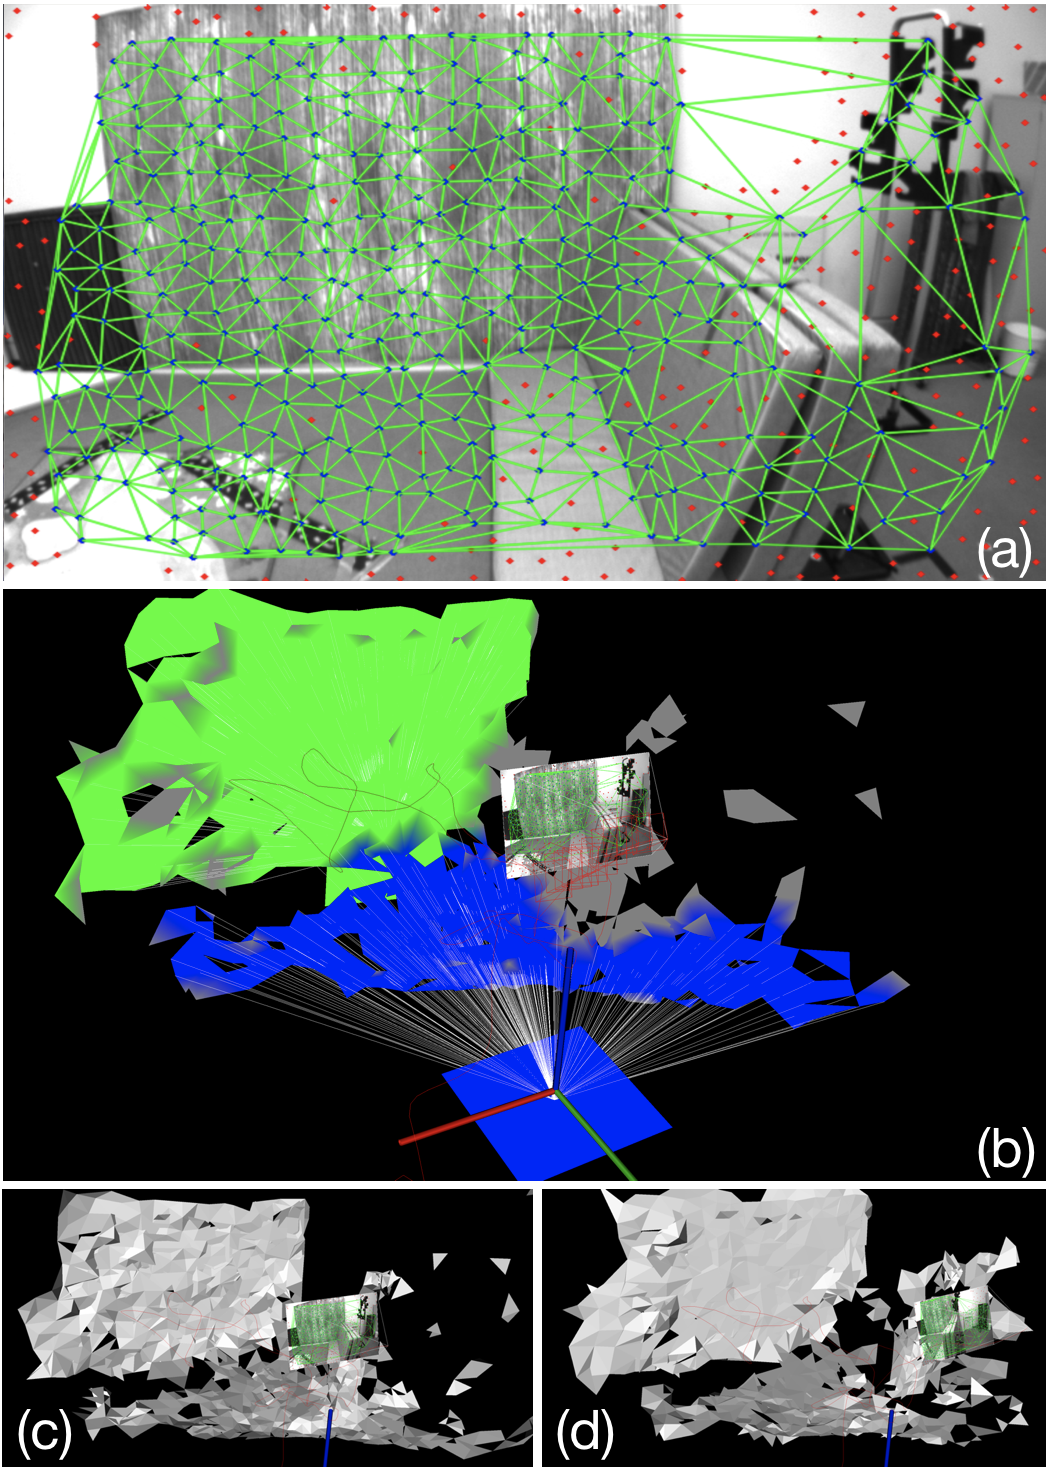
\includegraphics[width=\columnwidth]{overview4.png}
  %\subcaption{Mesh estimate without enforcing co-planarity constraints.}
  %\subcaption{Mesh estimate when enforcing co-planarity constraints.}
  \caption{We propose a VIO pipeline that incrementally builds a 3D mesh of the environment starting from (a) a 2D Delaunay triangulation of keypoints. We also detect and enforce \emph{structural regularities}, c.f.~(b) planar walls (green) and floor (blue). The bottom row in the figure compares the mesh constructed
  (c) without and (d) with structural regularities.\vspace{-5mm}}
  %Subfigures (c) and (d) show the mesh model  }
  %Visual comparison of the mesh with (bottom) and without (top) co-planarity constraints enforced.}
  \label{fig:intro}
\end{figure}

% Drop letter for first word of the Introduction
% Use only for final version.
% In recent years, great progress has been achieved using visual and inertial information (\cite{Mourikis07icra,Leutenegger15ijrr,Forster17troOnmanifold}).
% Unfortunately, these systems have nowadays two limitations that we want to address in this work, and which we detail below.
 \IEEEPARstart{R}{ecent} advances in VIO are enabling a wide range of applications, ranging from
 virtual and augmented reality to agile drone navigation~\cite{SayreMcCord18icra}.
 %Those applications are characterized by the need for low-latency estimates to be computed on computationally-constrained platforms, hence they demand for lightweight algorithms and implementations.

{\bf Contributions.}
In this paper, we propose to \emph{incrementally build a 3D mesh restricted to the receding horizon of the VIO optimization.}
In this way, we can map larger areas than a per-frame approach, while memory footprint and computational complexity associated to the mesh remain bounded.

{\bf Paper Structure.}
Section~\ref{sec:mathematical_formulation} presents the mathematical formulation of our approach, and discusses the implementation of %both %discussing both % the structure of our
our VIO front-end and back-end. % of our VIO.
Section~\ref{sec:results} reports and discusses the experimental results and comparison against related work. Section~\ref{sec:conclusions} concludes the paper.